\section{Algorithm}
\label{sec:MAMT:alg}

The key difference of this problem, compared against the popular definition of supervised problems, is that while our label ``0"s (or most of them, if not all) are reliable since we know there is not similar failure happened at those time or assets, our label ``1"s are uncertain and even most of them could be wrong. In this section we introduce our framework to solve this problem, which consists of supervised feature selection and dynamic and directional label propagation. 

\subsection{Supervised Feature Selection}
\label{sec:MAMT:alg:fea_sel} 
Intuitively, the requirement of failure signature analytics makes it closely connected to supervised feature selection. Thereby we first introduce a representative feature selection method based on  $\ell_{2,1}$ norm regularization ~\cite{liu2009multi} as our baseline feature selection algorithm. 

\begin{align}
\label{eq1:MAMT:l21}
& \min_{W} \| W^\top X - Y\|_F^2 + \alpha\|W\|_{2,1}, 
\end{align}
where $X \in \mathbb{R}^{m \times n}$ is the input dataset with $n$ samples and $m$ features, and $Y \in \mathbb{R}^{1 \times n}$ is the label vector in a binary classes setting with ``1" means the corresponding sample is considered as interesting and ``0" means it is normal sample. The final output $W \in \mathbb{R}^{m \times 1}$ gives a feature weighting vector represents the importance of each feature to the classification. 

The problem in Eq.\ref{eq1:MAMT:l21} can be interpreted as a generalized $\ell_{2,1}$ norm regularization problem~\cite{liu2009multi}, where the first term is a smooth convex loss function, and the second term controls the capacity of $W$ and also ensures that $W$ is sparse in rows, with the parameter $\alpha$ controlling the sparsity of $W$.   

\subsection{Dynamic and Directional Label Propagation}
\label{sec:MAMT:alg:lbl_ppg} 
As we mentioned earlier, what makes this problem unique to the popular feature selection, is that the label vector $Y$  is not able to be relied on. In some application cases it could be over $90\%$ mislabeled. Given such serious noisy labeling situation, the popular feature selection, and even the existing work on handling noisy labels ~\cite{tang2013coselect, frenay2014estimating} will easily fail since their assumption is only a small portion of labels are wrong. 

Here we introduce a Dynamic and Directional Label Propagation which can iteratively filter out wrong labels while maintaining those right ones. We start off by briefly describing the classic Label Propagation technique~\cite{wang2008graph, nie2010general}.  Consider a regularization framework on graph, the cost function associated with label propagation of $Y$ is defined as
\begin{align}
\label{eq1:MAMT:lbl_ppg}
& \min_{Y}  \sum_{i,j=1}^n \tilde{A}_{ij}\|Y_i-Y_j\|_F^2+\mu\sum_{i=1}^n\|Y_i-E_i\|^2,
\end{align}
where $Y \in \mathbb{R}^{1 \times n}$ is the label vector in a binary classes setting with ``1" means the corresponding sample is considered as interesting and ``0" means it is normal sample, $E \in \mathbb{R}^{1 \times n}$ is the label initialization, and $\tilde{A} \in \mathbb{R}^{n \times n}$  is a normalized affinity matrix.  The problem in Eq.\ref{eq1:MAMT:lbl_ppg} can be interpreted as a trade-off optimization problem, where the first term is a global smoothness meaning that two close samples should share the same labels, and the second term is a local fitness meaning that the final label should not be dramatically different from the initial seed, with parameter $\mu$ controlling the trade-off.  Label Propagation has strong connection with random walk, in the way that the label propagate out with the process of random walk~\cite{nie2010general}, which built upon a stable transition probability among samples. Figure~\ref{fig:MAMT:lbl_ppg:cls} shows the illustration of classic label propagation in a binary setting. We can see that given the initial label seed and a well constructed graph, the final label shows good classification result. 

\begin{figure}[htb]
\centering
\subfigure[classic label propagation]{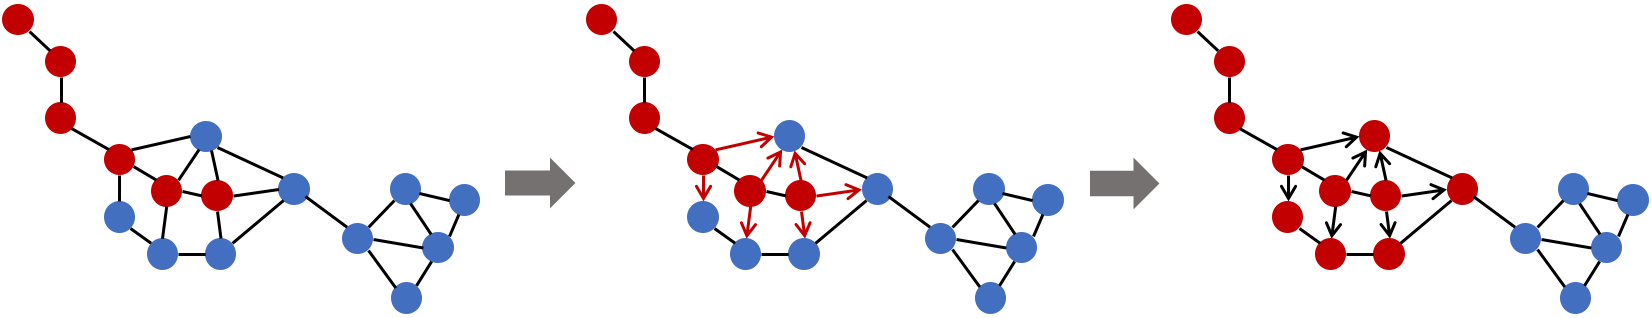
\includegraphics[width=3.3in]{pics/classic_label_propagation} \label{fig:MAMT:lbl_ppg:cls}}
\subfigure[Directional Label Propagation]{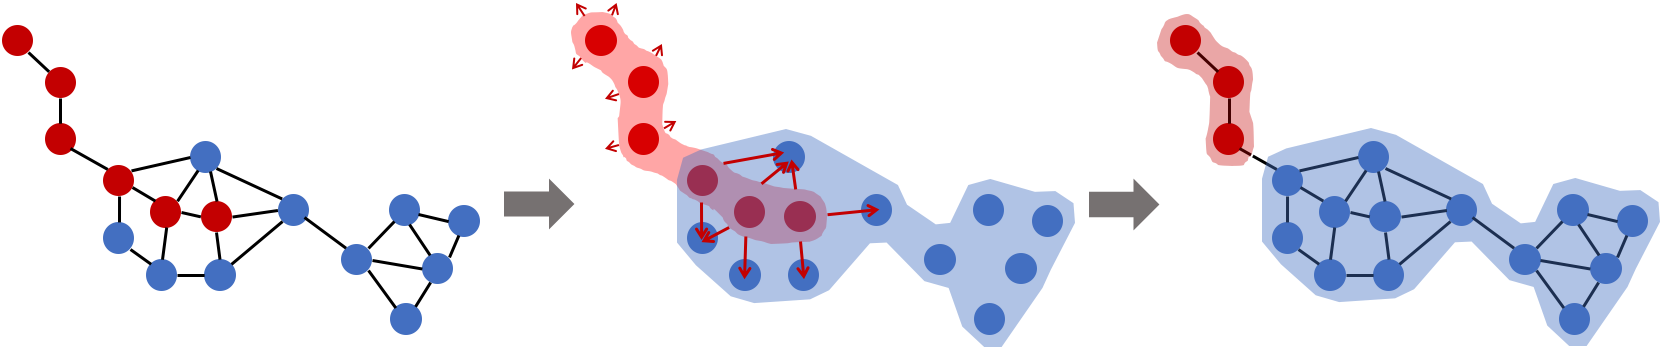
\includegraphics[width=3.3in]{pics/directional_label_propagation} \label{fig:MAMT:lbl_ppg:drc}}
\caption{Illustration of classic and our proposed label propagation. Red indicates the samples labeled as ``1" and blue as the ``0". }
\label{fig:MAMT:lbl_ppg}
\end{figure}

However, we have a different purpose in our problem setting:  \textbf{our goal is more on filtering out the wrong ``1" rather than expanding the right ``1"}.  Therefore, instead of constructing an omnidirectional random walk,  we model the propagation through a directional random walk as shown in Figure~\ref{fig:MAMT:lbl_ppg:drc}. Given the whole dataset as $\textbf{X} = [\textbf{X}_\textbf{a}, \textbf{X}_\textbf{b}] \in \mathbb{R}^{m \times n}$ with $m$ features and $n$ samples, and $\textbf{X}_\textbf{a} \in \mathbb{R}^{m \times a}$ is initially labeled as ``1" while $\textbf{X}_\textbf{b} \in \mathbb{R}^{m \times b}$ as ``0", we can construct a similarity matrix $A \in \mathbb{R}^{n \times n}$. We split matrix $A$ into $4$ blocks
\begin{align}            
\label{eq1:MAMT:A_block:01}
A = 
\begin{bmatrix}
A_{aa}&A_{ab}\\
A_{ba}&A_{bb}
\end{bmatrix},
\end{align}
where $A_{aa}$ describes the transition within $\textbf{X}_\textbf{a}$ and $A_{ab}$ describes the transition from $\textbf{X}_\textbf{a}$ to $\textbf{X}_\textbf{b}$ and so forth. 

In our problem setting, we assume that the samples in $\textbf{X}_\textbf{a}$ that labeled incorrectly in the initial seed are closed to (partial of) $\textbf{X}_\textbf{b}$ on all the feature subspace, and only those labeled correctly as ``1" are separable from $\textbf{X}_\textbf{b}$ in certain feature subspace. Therefore in a specifically designed label propagation, we hope the wrong ``1" is propagated out to its ``0" neighborhood and the right ``1" can be maintained. Detailedly speaking, we allow the ``1" labels propagate from $\textbf{X}_\textbf{a}$ to $\textbf{X}_\textbf{b}$ only, but not propagate back to $\textbf{X}_\textbf{a}$. Also we do not pay attention to the propagation within $\textbf{X}_\textbf{b}$ since no relevant event happened here and all these samples are assumed to be normal. Furthermore, we only allow self-loop exist in $\textbf{X}_\textbf{a}$ so the right ``1" can be conserved even there is high density in $\textbf{X}_\textbf{a}$. Therefore matrix $A$ is redefined as 
\begin{align}            
\label{eq1:MAMT:A_block:02}
A = 
\begin{bmatrix}
\mathrm{diag}(A_{aa})&A_{ab}\\
\textbf{0}_{ba}&\textbf{0}_{bb}
\end{bmatrix},
\end{align}  
where the lower part of $A$ are set to be $\textbf{0}$ matrix. Figure~\ref{fig:MAMT:lbl_ppg:drc} shows the illustration of our proposed Directional Label Propagation. We can see that given directional control, the wrong labels are ``flipped" and only the right ones conserved. 

\subsection{Our Proposed Framework}
\label{sec:MAMT:alg:framework} 
With our solutions to both feature side and label side, we are ready to introduce the Multi-view Failure Analysis on Multivariate Time-series Data (MAMT) framework. Considering both selecting the key feature (Eq.\ref{eq1:MAMT:l21}) and rectifying the labels (Eq.\ref{eq1:MAMT:lbl_ppg}), MAMT is to solve the following optimization 
\begin{align*}
\label{eq1:MAMT:mamt}
\mathcal{M}(W, \hat{Y}) &= \min_{W, \hat{Y}}  \| W^\top XB - \hat{Y}B\|_F^2 + \alpha\|W\|_{2,1} + \gamma\|\hat{Y}\|_{2,1}\\&+ \delta\bigg[\sum_{i,j=1}^n \tilde{A}_{ij}\|\hat{Y}_i-\hat{Y}_j\|_F^2+\mu\sum_{i=1}^n\|\hat{Y}_i-E_i\|^2\bigg],
\end{align*}
where $\hat{Y} = Y \circ E$ is the Hadamard product of $Y$ and $E$, while 
$E = [\textbf{1}_a, \textbf{0}_b] \in \mathbb{R}^{1 \times n}$ is the initial labels with $\textbf{1}_a = [1,1,...,1] \in \mathbb{R}^{1 \times a}$ corresponds to $\textbf{X}_\textbf{a}$ and $\textbf{0}_b = [0,0,...,0] \in \mathbb{R}^{1 \times b}$ corresponds to $\textbf{X}_\textbf{b}$, and $B = \mathrm{diag}([\beta\textbf{1}_a, \textbf{1}_b])$ is the sample weights in a diagonal format. The reason of bringing $\hat{Y}$ is because we want to ``compress" the label of $\textbf{X}_\textbf{b}$ all the time, and the reason of bringing $B$ is to handle the imbalance problem between $\textbf{X}_\textbf{a}$ and $\textbf{X}_\textbf{b}$. Please note that we also bring in a  $\ell_{2,1}$ norm regularization on $\hat{Y}$ to emphasize its scarcity in the final solution. In Section \ref{sec:MAMT:alg:proof_early} we will verify that the $\mathcal{M}(W, \hat{Y})$ is joinly convex with $W$ and $\hat{Y}$. 
 
It is difficult to optimize $W$ and $\hat{Y}$ simultaneously. Therefore we adopt an alternating optimization to solve this problem, which works well for a number of practical optimization problems\cite{feng2012adaptive, tang2013coselect}. 

\smallskip
\noindent\textbf{Given $\hat{Y}$, optimize $W$.}

\smallskip
\noindent\textbf{Given $W$, optimize $\hat{Y}$.}

\subsection{\color{red}{Proof and Early Stopping} }
\label{sec:MAMT:alg:proof_early} 

\subsection{Whole algorithm}
\label{sec:MAMT:alg:alg} 